\documentclass{beamer}

\mode<presentation> {

%\usetheme{default}
%\usetheme{AnnArbor}
%\usetheme{Antibes}
%\usetheme{Bergen}
%\usetheme{Berkeley}
%\usetheme{Berlin}
%\usetheme{Boadilla}
%\usetheme{CambridgeUS}
%\usetheme{Copenhagen}
%\usetheme{Darmstadt}
%\usetheme{Dresden}
%\usetheme{Frankfurt}
%\usetheme{Goettingen}
%\usetheme{Hannover}
%\usetheme{Ilmenau}
%\usetheme{JuanLesPins}
%\usetheme{Luebeck}
\usetheme{Madrid}
%\usetheme{Malmoe}
%\usetheme{Marburg}
%\usetheme{Montpellier}
%\usetheme{PaloAlto}
%\usetheme{Pittsburgh}
%\usetheme{Rochester}
%\usetheme{Singapore}
%\usetheme{Szeged}
%\usetheme{Warsaw}


%\usecolortheme{albatross}
%\usecolortheme{beaver}
%\usecolortheme{beetle}
%\usecolortheme{crane}
%\usecolortheme{dolphin}
%\usecolortheme{dove}
%\usecolortheme{fly}
%\usecolortheme{lily}
%\usecolortheme{orchid}
%\usecolortheme{rose}
%\usecolortheme{seagull}
%\usecolortheme{seahorse}
%\usecolortheme{whale}
%\usecolortheme{wolverine}

%\setbeamertemplate{footline} % To remove the footer line in all slides uncomment this line
%\setbeamertemplate{footline}[page number] % To replace the footer line in all slides with a simple slide count uncomment this line

%\setbeamertemplate{navigation symbols}{} % To remove the navigation symbols from the bottom of all slides uncomment this line
}

\usepackage{graphicx} % Allows including images
\usepackage{booktabs} % Allows the use of \toprule, \midrule and \bottomrule in tables
\usepackage{amsfonts}
\usepackage{mathrsfs, bbold}
\usepackage{amsmath,amssymb,graphicx}
\usepackage{mathtools} % gather
\usepackage[export]{adjustbox} % right-aligned graphics

% argmax
\DeclareMathOperator*{\argmax}{arg\,max}

%----------------------------------------------------------------------------------------
%	TITLE PAGE
%----------------------------------------------------------------------------------------

\title["13"]{13: Modal And Distributional Approximations}

\author{Taylor} 
\institute[UVA] 
{
University of Virginia \\
\medskip
\textit{} 
}
\date{} 

\begin{document}
%----------------------------------------------------------------------------------------

\begin{frame}
\titlepage 
\end{frame}

%----------------------------------------------------------------------------------------
\begin{frame}
\frametitle{Introduction}

We mention:
\begin{enumerate}
\item a few ways to find the posterior mode
\item how to approximate a posterior using a mode 
\item slightly more involved ways to approximate your posterior
\end{enumerate}

% For various reasons, we also frequently split up our parameters into two groups: $\theta = (\gamma, \phi)$.


\end{frame}

%----------------------------------------------------------------------------------------
\begin{frame}
\frametitle{Newton's Method aka the Newton-Raphson algorithm}

Based on a first-order approximation of the first derivative of the log-likelihood.
\newline

Approximate $L'(\theta) = (\log p(\theta \mid y))'$ as
$$
\mathbf{0} \overset{\text{set}}{=}  L'(\theta + \delta \theta) \approx L'(\theta ) + L''(\theta)(\delta \theta) 
$$
rearranges to 
$$
\delta \theta  =  - [L''(\theta)]^{-1} L'(\theta ) 
$$

\begin{block}{Newton's Method}
Repeat the following iteration until convergence:
\[
\theta^{t} = \theta^{t-1} - [L''(\theta^{t-1})]^{-1} L'(\theta^{t-1} ) 
\]
\end{block}

\end{frame}

%----------------------------------------------------------------------------------------
\begin{frame}
\frametitle{Newton's Method aka the Newton-Raphson algorithm}


\begin{block}{Newton's Method}
Repeat the following iteration until convergence:
\[
\theta^{t} = \theta^{t-1} - [L''(\theta^{t-1})]^{-1} L'(\theta^{t-1} ) 
\]
\end{block}

Notes:
\begin{enumerate}
\item easily handles unnormalized densities
\item starting value is important because it is not guaranteed to converge from everywhere
\item The derivatives can be determined analytically or numerically
\end{enumerate}

\end{frame}

%----------------------------------------------------------------------------------------
\begin{frame}[fragile]
\frametitle{Quasi-Newton and conjugate gradient methods}

Notes:
\begin{enumerate}
\item Quasi-Newton methods (approximate second derivatives) are available when second derivatives are too costly or unavailable
\item "Broyden-Fletcher-Goldfarb-Shanno" is a common example of a Quasi-Newton method
\item in \verb|R|: \verb|optim(2.9,F,method=``BFGS")|
\item conjugate-gradient methods only use gradient information, but they are for models of the form $\Vert A \theta - b \Vert_2$ (also handled by \verb|optim()| )
\item compared with the two above, they generally require more iterations, but use less computation per iteration and less storage
\end{enumerate}

\end{frame}

%----------------------------------------------------------------------------------------
\begin{frame}[fragile]
\frametitle{Numerical computation of derivatives}

In \verb|optim|, if you don't provide a function to calculate the gradient, then it uses a finite-difference approximation:

$$
L_i'(\theta) = \frac{dL}{d\theta_i } \approx \frac{L(\theta + \delta_i e_i ) - L(\theta - \delta_i e_i )}{2 \delta_i }
$$
and
\begin{align*}
L_{ij}''(\theta) &= \frac{d^2L}{d\theta_i d\theta_j } \\
&\approx \frac{ L_i'(\theta + \delta_j e_j ) - L_i'(\theta - \delta_j e_j )}{2 \delta_j } \\
\end{align*}
where $e_j$ is the vector of all zeros except for a $1$ in the $j$th spot, and $\delta_j$ is a small number (\verb|optim|'s default is $1e-3$)
\end{frame}

%----------------------------------------------------------------------------------------
\begin{frame}[fragile]
\frametitle{Gaussian approximations}

Once the mode or modes have been found (perhaps after including a boundary-avoiding prior distribution as discussed in section 13.2, or after transforming the parameters appropriately), we can construct an approximation based on the multivariate normal distribution. 
\newline

Let $\hat{\theta}$ be the mode, then 
$$
p(\theta \mid y) \approx N(\hat{\theta}, V_{\theta})
$$
where 
$$
V_{\theta} = \left[- \frac{d^2 \log p(\theta \mid y) }{d\theta^2}\bigg\rvert_{\theta = \hat{\theta}} \right]^{-1}
$$
is calculated exactly or approximated using the formula from a few slides ago.

\end{frame}


%----------------------------------------------------------------------------------------
\begin{frame}[fragile]
\frametitle{Example}

From chapter 3:
\begin{enumerate}
\item $p(y_i \mid \mu, \sigma^2) = \text{Normal}(\mu, \sigma^2)$
\item $p(\mu, \sigma^2) \propto 1/\sigma^2$
\end{enumerate}
\[
p(\mu, \sigma^2 \mid y) \propto (\sigma^2)^{-(n+2)/2}\exp\left[ - \frac{1}{2\sigma^2}\left\{(n-1)  s^2 + n(\bar{y} - \mu)^2 \right\} \right]
\]



\end{frame}

%----------------------------------------------------------------------------------------
\begin{frame}[fragile]
\frametitle{Example}

\[
p(\mu, \sigma^2 \mid y) \propto (\sigma^2)^{-(n+2)/2}\exp\left[ - \frac{1}{2\sigma^2}\left\{(n-1)  s^2 + n(\bar{y} - \mu)^2 \right\} \right]
\]

Letting $\theta = \log \sigma$, $p(\mu, \theta \mid y)$ is proportional to
\[
\exp[-n\theta]\exp\left[ - \frac{1}{2\exp[2\theta]}\left\{(n-1)  s^2 + n(\bar{y} - \mu)^2 \right\} \right] 
\]

So $\log p(\mu, \theta \mid y)$ is 
$$
constant -n\theta - .5\exp(-2\theta)\left[(n-1)  s^2 + n(\bar{y} - \mu)^2 \right]
$$
and $L'(\theta) = \left[\begin{array}{c}
\exp(-2\theta)(\bar{y}-\mu)n \\ -n + \exp(-2\theta)\left[(n-1)  s^2 + n(\bar{y} - \mu)^2 \right]
\end{array}\right]$

\end{frame}

%----------------------------------------------------------------------------------------
\begin{frame}[fragile]
\frametitle{Example}

Warning: \verb|optim| *minimizes*, so we use $-\log p(\mu, \theta \mid y)$ 
$$
n\theta + .5\exp(-2\theta)\left[(n-1)  s^2 + n(\bar{y} - \mu)^2 \right]
$$
and 
$$
-L'(\theta) = \left[\begin{array}{c}
-\exp(-2\theta)(\bar{y}-\mu)n \\ 
n - \exp(-2\theta)\left[(n-1)  s^2 + n(\bar{y} - \mu)^2 \right]
\end{array}\right]
$$

\begin{verbatim}
# if gr left blank, finite difference approx. used
optim_results <- optim(par = c(5, 0), 
                       fn = neg_log_unnorm_post, 
                       gr = gradient, 
                       method = "BFGS", 
                       hessian = T)
\end{verbatim}
See \verb|mode_finding_examples.r|

\end{frame}

%----------------------------------------------------------------------------------------
\begin{frame}[fragile]
\frametitle{Example}

\begin{center}
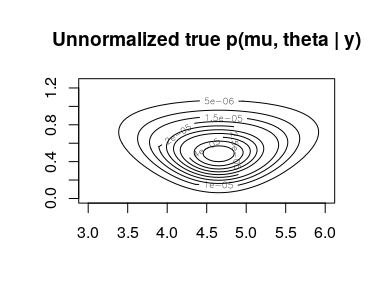
\includegraphics[width=105mm]{unnorm_true}
\end{center}

\end{frame}

%----------------------------------------------------------------------------------------
\begin{frame}[fragile]
\frametitle{Example}

\begin{center}
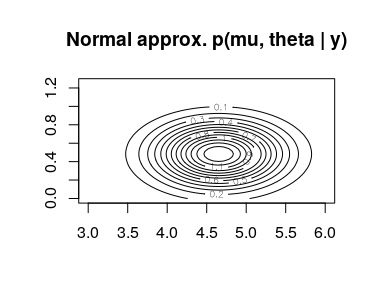
\includegraphics[width=105mm]{norm_approx}
\end{center}

\end{frame}

%----------------------------------------------------------------------------------------
\begin{frame}[fragile]
\frametitle{Gaussian approximations: Laplace's Method}

If you want approximations to posterior *expectations* (say $E[h(\theta) \mid y]$), then you might consider Laplace's method, which is based on second-order Taylor approximations of the functions:
\begin{enumerate}
\item $u_1(\theta) = \log[h(\theta)q(\theta \mid y)]$
\item $u_2(\theta) = \log q(\theta \mid y)$
\end{enumerate}
where $p(\theta \mid y) = q(\theta \mid y) / \int q(\theta \mid y)\text{d}\theta$. 
\newline

Both are centered at maximizing values: $\theta_0^1, \theta_0^2$, and this assumes $h$s are twice continuously differentiable.
\newline

Idea:
$$
\frac{\int h(\theta)q(\theta \mid y) \text{d}\theta}{\int q(\theta \mid y) \text{d}\theta } = \frac{\int \exp\left[ \log h(\theta) + \log q(\theta \mid y) \right] \text{d}\theta}{ \int \exp\left[ \log q(\theta \mid y) \right] \text{d}\theta }
$$


\end{frame}


%----------------------------------------------------------------------------------------
\begin{frame}[fragile]
\frametitle{Gaussian approximations: Laplace's Method}

Exponentiating and integrating (typo on page 318?)

\begin{align*}
u(\theta) &\approx u(\theta_0) + (\theta - \theta_0)^Tu'(\theta_0) + \frac{1}{2}(\theta - \theta_0)^T u''(\theta_0)(\theta - \theta_0) \\
&= u(\theta_0) + \frac{1}{2}(\theta - \theta_0)^T u''(\theta_0)(\theta - \theta_0)
\end{align*}

gives us

\begin{align*}
\int \exp[ u(\theta) ] \text{d}\theta &\approx \int \exp[ u(\theta_0)  + \frac{1}{2}(\theta - \theta_0)^T u''(\theta_0)(\theta - \theta_0) ] \text{d}\theta \\
&= \exp [u(\theta_0)] \int \exp\left[\frac{1}{2}(\theta - \theta_0)^T u''(\theta_0)(\theta - \theta_0) \right] \text{d}\theta \\
&= \exp [u(\theta_0)] \int \exp\left[-\frac{1}{2}(\theta - \theta_0)^T \{-u''(\theta_0)\}(\theta - \theta_0) \right] \text{d}\theta \\
&= \exp [u(\theta_0)] (2\pi)^{d/2} \det[-u''(\theta_0)]^{-1/2}
\end{align*}


\end{frame}

%----------------------------------------------------------------------------------------
% \begin{frame}[fragile]
% \frametitle{Gaussian approximations: Laplace's Method}
% 
% Looking at the numerator:
% 
% \begin{align*}
% \int \exp\left[ \log h(\theta) + \log q(\theta \mid y) \right] \text{d}\theta &= 
% \end{align*}

% \begin{align*}
% \exp[ u(\theta) ] &\approx \exp[ u(\theta_0) + (\theta - \theta_0)^Tu'(\theta_0) + \frac{1}{2}(\theta - \theta_0)^T u''(\theta_0)(\theta - \theta_0) ] \\
% &= \exp [u(\theta_0)]\exp\left[\frac{1}{2}(\theta - \theta_0)^T u''(\theta_0)(\theta - \theta_0) \right] \\
% &= \exp [u(\theta_0)]\exp\left[-\frac{1}{2}(\theta - \theta_0)^T \{-u''(\theta_0)\}(\theta - \theta_0) \right]
% 
% Looking at the numerator:
% \begin{align*}
% \int \exp\left[ u_1(\theta)\right] \text{d}\theta \\
% &\approx \exp\left[ u(\theta_0)\right] \int\exp\left[ \frac{1}{2}(\theta - \theta_0)^T u''(\theta_0)(\theta - \theta_0)\right] \text{d}\theta \\
% &= h(\theta_0)p(\theta_0 \mid y) \int\exp\left[ - \frac{1}{2}(\theta - \theta_0)^T\left[- u''(\theta_0)\right](\theta - \theta_0)\right] \text{d}\theta \\
% &= h(\theta_0)p(\theta_0 \mid y) (2 \pi)^{d/2} \det\left(\left[- u''(\theta_0)\right]^{-1}\right)^{1/2} \\
% &= h(\theta_0)p(\theta_0 \mid y) (2 \pi)^{d/2} \det\left(\left[- u''(\theta_0)\right]\right)^{-1/2}
% \end{align*}
% 
% \end{frame}


%----------------------------------------------------------------------------------------
\begin{frame}[fragile]
\frametitle{Gaussian approximations}

The book has a few more generalizations that we don't address:

\begin{enumerate}
\item approximating multimodal distributions with normal mixtures
\item approximating multimodal distributions with t mixtures
\end{enumerate}

\end{frame}


%----------------------------------------------------------------------------------------
\begin{frame}[fragile]
\frametitle{The EM Algorithm}

The {\bf expectation-maximization algorithm} finds the argument that maximizes the marginal posterior. It's useful in situations where there is missing data in a model (e.g. hierarchical models, factor models, hidden markov models, state space models, etc.). 
\newline

It folows the following steps
\begin{enumerate}
\item replace missing values by their expectations given the guessed parameters, 
\item estimate parameters assuming the missing data are equal to their estimated values, 
\item re-estimate the missing values assuming the new parameter estimates are correct,
\item re-estimate parameters, 
\end{enumerate}
and so forth, iterating until convergence.

\end{frame}


%----------------------------------------------------------------------------------------
\begin{frame}[fragile]
\frametitle{The EM Algorithm}

Call $\theta = (\gamma, \phi)$. You're interested in the mode of $p(\phi \mid y)$. Typically, $\gamma$ is ``hidden data."
\newline

$$
\log p(\phi \mid y) = \log \frac{p(\gamma, \phi \mid y)}{p(\gamma \mid \phi, y)} = \log \underbrace{p(\gamma, \phi \mid y)}_{ \text{joint posterior} } - \log \underbrace{p(\gamma \mid \phi, y)}_{\text{conditional posterior }}
$$
\pause

taking expectations on both sides with respect to $p(\gamma \mid \phi^{\text{old}}, y)$ yields:
$$
\log p(\phi \mid y) =  E\left[ \log p(\gamma, \phi \mid y) \mid \phi^{\text{old}}, y \right] - E\left[\log p(\gamma \mid \phi, y) \mid \phi^{\text{old}}, y \right]
$$

% exercise 13.6 !



\end{frame}

%----------------------------------------------------------------------------------------
\begin{frame}[fragile]
\frametitle{The EM Algorithm}

We iteratively use the middle term in
$\log p(\phi \mid y) =  E\left[ \log p(\gamma, \phi \mid y) \mid \phi^{\text{old}}, y \right] - E\left[\log p(\gamma \mid \phi, y) \mid \phi^{\text{old}}, y \right]$.

\begin{block}{The Q quantity in the ``E" step}

$$
Q(\phi \mid \phi^{\text{old}}) = E\left[ \log p(\gamma, \phi \mid y) \mid \phi^{\text{old}}, y \right]
$$
\end{block}
\pause

\begin{block}{The EM algorithm}

Repeat the following until convergence:
\begin{enumerate}
\item E-step: calculate $Q(\phi \mid \phi^{\text{old}})$
\item M-step: replace $\phi^{\text{old}}$ with $\argmax Q(\phi \mid \phi^{\text{old}})$
\end{enumerate}
\end{block}
\end{frame}

%----------------------------------------------------------------------------------------
\begin{frame}[fragile]
\frametitle{The EM Algorithm}

If we follow this strategy, $\log p(\phi \mid y)$ increases at every iteration:
\begin{align*}
\log p(\phi \mid y) &=  E\left[ \log p(\gamma, \phi \mid y) \mid \phi^{\text{old}}, y \right] - E\left[\log p(\gamma \mid \phi, y) \mid \phi^{\text{old}}, y \right]\\
&= Q(\phi \mid \phi^{\text{old}}) - E\left[\log p(\gamma \mid \phi, y) \mid \phi^{\text{old}}, y \right] \tag{defn. Q} \\
&\ge Q(\phi \mid \phi^{\text{old}}) - E\left[\log p(\gamma \mid \phi^{\text{old}}, y) \mid \phi^{\text{old}}, y \right] \tag{HW}
\end{align*}
\pause

So 
\begin{align*}
&\log p(\phi^{\text{new}} \mid y) - \log p(\phi^{\text{old}} \mid y) \\
&= \log p(\phi^{\text{new}} \mid y) - \left\{Q(\phi^{\text{old}} \mid \phi^{\text{old}}) - E\left[\log p(\gamma \mid \phi^{\text{old}}, y) \mid \phi^{\text{old}}, y \right] \right\} \\
&\ge Q(\phi^{\text{new}} \mid \phi^{\text{old}}) - E\left[\log p(\gamma \mid \phi^{\text{old}}, y) \mid \phi^{\text{old}}, y \right] \\
&\hspace{10mm} - \left\{Q(\phi^{\text{old}} \mid \phi^{\text{old}}) - E\left[\log p(\gamma \mid \phi^{\text{old}}, y) \mid \phi^{\text{old}}, y \right] \right\} \\
&= Q(\phi^{\text{new}} \mid \phi^{\text{old}}) - Q(\phi^{\text{old}} \mid \phi^{\text{old}})
\end{align*}

\end{frame}

%----------------------------------------------------------------------------------------
\begin{frame}[fragile]
\frametitle{The EM Algorithm}

Notes:
\begin{enumerate}
\item The EM algo isn't inherently Bayesian. It can also be used to accomplish maximum likelihood estimation.
\item The expectation of $\log p(\gamma, \phi \mid y)$ is usually easy to compute because it is a sum, and might only depend on sufficient statistics
\item The EM algorithm implicitly deals with parameter constraints in the M-step
\item The EM algorithm is parameterization independent
\item The *Generalized* EM (GEM) just increases $Q$ instead of maximizing it.
\item The book describes many generalizations, in addition to this one
\item You might find multiple modes if you start from multiple starting points (using mixture approximations afterwards)
\item if you can, debug by printing $\log p(\phi^i \mid y)$ at every iteration and make sure it increases monotonically
\end{enumerate}

\end{frame}


%----------------------------------------------------------------------------------------
\begin{frame}[fragile]
\frametitle{Variational Inference}

{\bf Variational inference} approximates an intractable posterior $p(\theta \mid y)$ with some chosen distribution $g(\theta \mid \phi)$ (e.g. multivariate normal).
\newline
\pause

We will assume this approximating distribution factors into $J$ components:
$$
g(\theta \mid \phi) = \prod_{j=1}^J g_j(\theta_j \mid \phi_j) = g_j(\theta_j \mid \phi_j)g_{-j}(\theta_{-j} \mid \phi_{-j}).
$$


We will find $\phi$ using an EM-like algorithm that minimizes Kullback-Leibler divergence.

\end{frame}

%----------------------------------------------------------------------------------------
\begin{frame}[fragile]
\frametitle{Variational Inference}

Kullback-Leibler divergence is ``reversed" this time:
\begin{align*}
KL(g || p) &= - \int \log \left( \frac{ p(\theta \mid y)}{g(\theta \mid \phi)} \right) g(\theta \mid \phi)\text{d}\theta  \\
&= - \int \log \left( \frac{ p(\theta, y)}{g(\theta \mid \phi)} \right) g(\theta \mid \phi)\text{d}\theta
+ \int \log p(y)g(\theta \mid \phi) \text{d}\theta \\
&= - \underbrace{\int \log \left( \frac{ p(\theta, y)}{g(\theta \mid \phi)} \right) g(\theta \mid \phi)\text{d}\theta}_{\text{variational lower bound}}
+  \log p(y) \\
\end{align*}

The term that we maximize (minimize the negative) is called the {\bf variational lower bound} aka the {\bf evidence lower bound} (ELBO).

\end{frame}

%----------------------------------------------------------------------------------------
\begin{frame}[fragile]
\frametitle{Variational Inference}

Every iteration, we cycle through all the hyper-parameters $\phi_1, \ldots, \phi_J$, and change them until convergence is reached.
\newline
\pause

Looking at $\phi_j$...
\begin{align*}
&\int \log \left( \frac{ p(\theta, y)}{g(\theta \mid \phi)} \right) g(\theta \mid \phi)\text{d}\theta \\
&=  \iint \left[\log p(\theta, y) - \log g_j(\theta_j \mid \phi_j) - \log g_{-j}(\theta_{-j} \mid \phi_{-j})\right]  \\
&\hspace{10mm} g_j(\theta_j \mid \phi_j)g_{-j}(\theta_{-j} \mid \phi_{-j})\text{d}\theta_{j}\text{d}\theta_{-j} \\
&=  \int \left[\int\log p(\theta, y)g_{-j}(\theta_{-j} \mid \phi_{-j}) \text{d}\theta_{-j}\right] g_j(\theta_j \mid \phi_j)\text{d}\theta_{j} \\
&- \int\log g_j(\theta_j \mid \phi_j)g_j(\theta_j \mid \phi_j)\text{d}\theta_j - \int \log g_{-j}(\theta_{-j} \mid \phi_{-j})g_{-j}(\theta_{-j} \mid \phi_{-j})\text{d}\theta_{-j} \\ 
&=  \int  \log \left(\frac{\tilde{p}(\theta_j)}{g_j(\theta_j \mid \phi_j)}  \right) g_j(\theta_j \mid \phi_j)\text{d}\theta_{j} + \text{constant} \tag{*}
\end{align*}

\end{frame}

%----------------------------------------------------------------------------------------
\begin{frame}[fragile]
\frametitle{Variational Inference}

We think of $\tilde{p}(\theta_j)$ as an unnormalized density 
$$
\log\tilde{p}(\theta_j) = \int\log p(\theta, y)g_{-j}(\theta_{-j} \mid \phi_{-j}) \text{d}\theta_{-j}
$$
because usually

\begin{align*}
\int \tilde{p}(\theta_j) \text{d}\theta_j &= \int \exp\left[ \int\log p(\theta, y)g_{-j}(\theta_{-j} \mid \phi_{-j}) \text{d}\theta_{-j}\right] \text{d}\theta_j \\
&\le \int \exp\left[ \log \int p(\theta, y)g_{-j}(\theta_{-j} \mid \phi_{-j}) \text{d}\theta_{-j}\right] \text{d}\theta_j \tag{Jensen's}\\
&= \iint  p(\theta, y)g_{-j}(\theta_{-j} \mid \phi_{-j}) \text{d}\theta_{-j} \text{d}\theta_j \\
&< \infty
\end{align*}

\end{frame}

%----------------------------------------------------------------------------------------
\begin{frame}[fragile]
\frametitle{Variational Inference}

\begin{block}{VI algorithm}
For $j=1,\ldots,J$ set $\phi_j$ so that $\log g_j(\theta_j \mid \phi_j)$ is equal to 
$$
\log\tilde{p}(\theta_j) = \int\log p(\theta, y)g_{-j}(\theta_{-j} \mid \phi_{-j}) \text{d}\theta_{-j}
$$
\end{block}

\end{frame}

%----------------------------------------------------------------------------------------
\begin{frame}[fragile]
\frametitle{Variational Inference: educational testing example}

When the parameters are $\alpha_1, \ldots, \alpha_8, \mu, \tau$, the log posterior is
$$
\log p(\theta \mid y) = \text{constant} - \frac{1}{2}\sum_{j=1}^8\frac{(y_j - \alpha_j)^2 }{\sigma^2_j } - 8 \log \tau - \frac{1}{2}\frac{1}{\tau^2}\sum_{j=1}^8(\alpha_j - \mu)^2
$$
and we assume
$$
g(\alpha_1, \ldots, \alpha_8, \mu, \tau) = g(\alpha_1) \times  \cdots \times g(\alpha_8) g(\mu) g(\tau).
$$

Let's reparameterize $\tau$ as $\tau^2$ and assume $g(\alpha_1), \ldots, g(\alpha_8) g(\mu)$ are all normal distributions, and $g(\tau^2)$ is an Inverse-Gamma.

  
\end{frame}


%----------------------------------------------------------------------------------------
\begin{frame}[fragile]
\frametitle{Variational Inference: example}


\begin{align*}
&\log g(\alpha_j) \\
&\overset{\text{set}}{=} \log\tilde{p}(\alpha_j) \\
&= \int\log p(\theta, y)g_{-j}(\theta_{-j}) \text{d}\theta_{-j} \\
&= - \frac{1}{2}\sum_{i=1}^8\frac{E_{-j}[(y_i - \alpha_i)^2 ] }{\sigma^2_i } - 8 E_{-j}[\log \tau] - \frac{1}{2} E_{-j}\left[\frac{1}{\tau^2}\right] \sum_{i=1}^8 E[(\alpha_i - \mu)^2 ] + c \\
&= - \frac{1}{2}\frac{(y_j - \alpha_j)^2 }{\sigma^2_j } -  \frac{1}{2} E_{-j}\left[\frac{1}{\tau^2}\right] E_{-j}[(\alpha_j - \mu)^2 ] + c' \\
&= - \frac{1}{2}\frac{(y_j - \alpha_j)^2 }{\sigma^2_j } -  \frac{1}{2} E_{-j}\left[\frac{1}{\tau^2}\right] (\alpha_j^2 - 2\alpha_j E_{-j}[\mu] ) ] + c''
\end{align*}
We are using linearity, independence, the data aren't random, and we're grouping all the terms that don't involve $\alpha_j$ into the constant.
\newline

So $g(\alpha_j) = $...
\end{frame}

%----------------------------------------------------------------------------------------
\begin{frame}[fragile]
\frametitle{Variational Inference: example}


For $\mu$:
\begin{align*}
\log\tilde{p}(\mu) &= \int\log p(\theta, y)g_{-j}(\theta_{-j} \mid \phi_{-j}) \text{d}\theta_{-j} \\
&= - \frac{1}{2}E_{-\mu}\left[ \frac{1}{\tau^2}\sum_{j=1}^8(\alpha_j - \mu)^2\right] + \text{constant} \\
&= - \frac{1}{2}E_{-\mu}\left[ \frac{1}{\tau^2} \right] \sum_{j=1}^8 \left( \mu^2 - 2 \mu E_{-\mu}[ \alpha_j] \right) + \text{constant} \\
&= - \frac{1}{2}E_{-\mu}\left[ \frac{1}{\tau^2} \right]  \left( 8 \mu^2 - 2 \mu \sum_{j=1}^8 E_{-\mu}[ \alpha_j] \right) + \text{constant}
\end{align*}

So $g(\mu) = $...
\end{frame}

%----------------------------------------------------------------------------------------
\begin{frame}[fragile]
\frametitle{Variational Inference: example}


For $\tau$ (not $\tau^2$):
\begin{align*}
\log\tilde{p}(\tau) &= \int\log p(\theta, y)g_{-j}(\theta_{-j} \mid \phi_{-j}) \text{d}\theta_{-j} \\
&= - 8 \log \tau - \frac{1}{2}\frac{1}{\tau^2} E_{-\tau}\left[ \sum_{j=1}^8(\alpha_j - \mu)^2 \right] + c \\
\end{align*}

So $g(\tau) \propto \tau^{-8} \exp\left[-\frac{\sum_jE_{-\tau}[(\alpha_j - \mu)^2]}{2 \tau^2} \right]$ which means $$
g(\tau^2) = (\tau^2)^{-(\frac{7}{2}+1)}\exp\left[-\frac{\sum_jE_{-\tau}[(\alpha_j - \mu)^2]}{2 \tau^2} \right]
$$
which is an InverseGamma$\left( \frac{7}{2}, \frac{\sum_jE_{-\tau}[(\alpha_j - \mu)^2]}{2 }\right)$
\end{frame}

%----------------------------------------------------------------------------------------
\begin{frame}[fragile]
\frametitle{Variational Inference: example}

To complete this example, we need to derive:
\begin{itemize}
\item for $g(\alpha_j)$: 
  \begin{enumerate}
  \item $E_{-j}\left[\frac{1}{\tau^2}\right] = E_{\tau^2}\left[\frac{1}{\tau^2}\right]$, 
  \item $ E_{-j}[\mu] = E_{\mu}[\mu]$ 
  \end{enumerate}
\item for $g(\mu)$: 
  \begin{enumerate}
  \item $E_{-\mu}[ \alpha_j] = E_{\alpha_j}[ \alpha_j]$, 
  \item $E_{-j}\left[\frac{1}{\tau^2}\right] = E_{\tau^2}\left[\frac{1}{\tau^2}\right]$ 
  \end{enumerate}
\item for $g(\tau^2)$: 
  \begin{enumerate}
  \item $\sum_jE_{-\tau}[(\alpha_j - \mu)^2] = \sum_jE_{\alpha_j,\mu}[(\alpha_j - \mu)^2]$, 
  \end{enumerate}
\end{itemize}

\end{frame}

%----------------------------------------------------------------------------------------
\begin{frame}[fragile]
\frametitle{Variational Inference: example}

\begin{center}
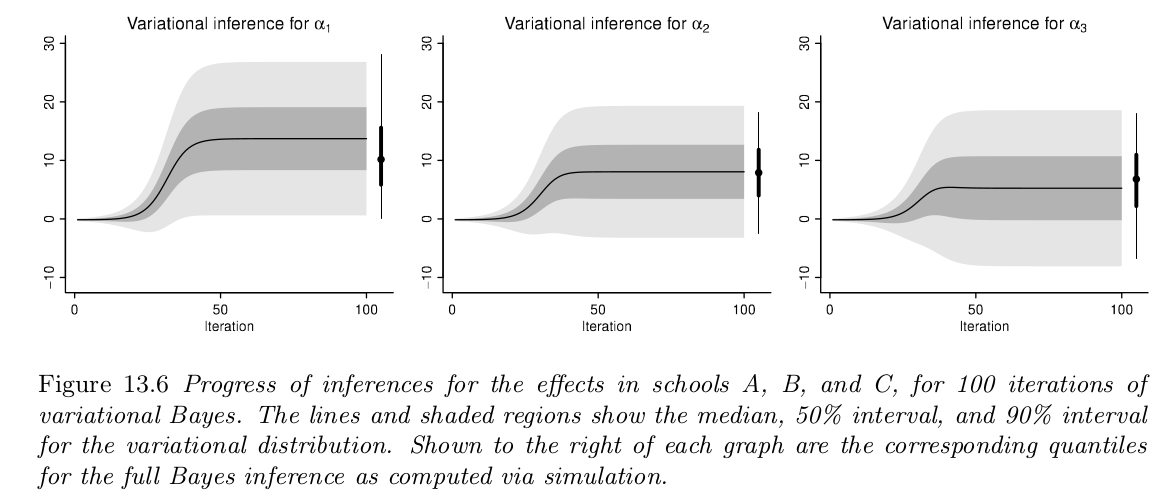
\includegraphics[width=120mm]{vi_convergence.png}
\end{center}

\end{frame}




%----------------------------------------------------------------------------------------
\begin{frame}[fragile]
\frametitle{Expectation Propagation: warmup}

$p(x \mid \theta)$ is in the exponential family if it can be written as  
$$
h(x)\exp\left[\eta(\theta)'T(x) - A(\theta) \right]
$$

Example:
$$
N(\theta \mid \mu, \sigma^2) = \frac{1}{\sqrt{2\pi\sigma^2}} \exp\left[-\frac{1}{2\sigma^2}\theta^2 + \frac{\mu}{\sigma^2}\theta - \frac{\mu^2}{2\sigma^2} \right]
$$
sufficient statistic: $(\theta^2,\theta)$

canonical/natural parameters: $(-\frac{1}{2\sigma^2}, \frac{\mu}{\sigma^2})$

\end{frame}
%----------------------------------------------------------------------------------------
\begin{frame}[fragile]
\frametitle{Expectation Propagation}

{\bf Expectation Propogation} is another deterministic iterative technique that approximates the posterior with a distribution that is in the exponential family. 
\newline

\begin{enumerate}
\item $p(\theta \mid y) = f(\theta) = \prod_{i=0}^{n} f_i(\theta)$
\item $g(\theta) = \prod_{i=0}^{n} g_i(\theta)$
\end{enumerate}

$f_0(\theta) = p(\theta)$, $f_1(\theta) = p(y_1 \mid \theta)$, ...
\newline

For more info: \url{https://arxiv.org/abs/1412.4869}
\end{frame}
%----------------------------------------------------------------------------------------
\begin{frame}[fragile]
\frametitle{Expectation Propagation}

The {\bf cavity distribution} is 
$$
g_{-i}(\theta) \propto g(\theta) / g_i(\theta),
$$
and the {\bf tilted distribution} is 
$$
g_{-i}(\theta) f_i(\theta).
$$

At each stage, we update $g_i(\theta)$ so that we ``target" $g_{-i}(\theta) f_i(\theta)$ with $g(\theta)$. 


\end{frame}

%----------------------------------------------------------------------------------------
\begin{frame}[fragile]
\frametitle{Expectation Propagation}

At each stage, we update $g_i(\theta)$ so that we ``target" $g_{-i}(\theta) f_i(\theta)$ with $g(\theta)$. 
\newline

Notice that
$$
\frac{\text{target}}{\text{``proposal"} } = \frac{g_{-i}(\theta) f_i(\theta)}{g(\theta)} = \frac{f_i(\theta)}{g_i(\theta)}.
$$

However, we cannot ignore the cavity distribution in each ``site" update. This is because we choose $g(\theta)$ so that its {\bf moments match} those of $g_{-i}(\theta) f_i(\theta)$. This is like choosing $g_i(\theta)$ to approximate $f_i(\theta)$ {\bf in the context of} $g_{-i}(\theta)$.

\end{frame}

%----------------------------------------------------------------------------------------
\begin{frame}[fragile]
\frametitle{Expectation Propagation}

If $g(\theta) = \text{Normal}(\mu, \Sigma)$, for each $i$ we change $\mu$ and $\Sigma$ by solving
$$
\mu \overset{\text{set}}{=} E_{\text{tilted }i}[\theta] 
$$
and
$$
\Sigma \overset{\text{set}}{=} \operatorname{Var}_{\text{tilted }i}[\theta] 
$$
where $E_{\text{tilted }i}[\theta] = \int \theta g_{-i}(\theta)f_i(\theta) \text{d}\theta $ and $\operatorname{Var}_{\text{tilted }i}[\theta] = \int (\theta-\mu)(\theta-\mu)' g_{-i}(\theta)f_i(\theta) \text{d}\theta $.
\newline

The hard part is integrating.
\end{frame}
%----------------------------------------------------------------------------------------
\begin{frame}[fragile]
\frametitle{Expectation Propagation: example}

Let $\theta$ be a vector of regression parameters for a logistic regression:
\begin{align*}
p(\theta \mid y) &\propto \prod_{i=1}^n p(y_i \mid \theta)p(\theta) \\
&= \prod_{i=0}^n f_i(\theta) \\
&= f_0(\theta) \prod_{i=1}^n [\text{invlogit}(X_i'\theta )]^{y_i}[1-\text{invlogit}(X_i'\theta)]^{m_i - y_i}
\end{align*}

and choose $g(\theta)$ to be $\text{Normal}(\mu, \Sigma)$

\end{frame}
%----------------------------------------------------------------------------------------
\begin{frame}[fragile]
\frametitle{Expectation Propagation: example}

We choose $g(\theta)$ to be $\text{Normal}(\mu, \Sigma)$:
\begin{align*}
g(\theta) 
&\propto \prod_{i=0}^n \exp\left[-\frac{1}{2}(\theta - \mu_i)'\Sigma^{-1}_i(\theta - \mu_i)  \right] \\
&\propto  \exp\left[-\frac{1}{2}\sum_{i=0}^n\left( \theta'\Sigma^{-1}_i\theta - 2 \mu_i' \Sigma^{-1}_i\theta \right) \right] \\
&=  \exp\left[-\frac{1}{2}\left( \theta'\left[\underbrace{ \sum_{i=0}^n \Sigma^{-1}_i}_{\Sigma^{-1} }\right] \theta - 2 \left[\underbrace{\sum_{i=0}^n\mu_i' \Sigma^{-1}_i}_{ \text{natural param 2} } \right]\theta \right) \right]
\end{align*}

Algorithmically, $\mu, \Sigma$ change at each iteration.
\end{frame}

%----------------------------------------------------------------------------------------
\begin{frame}[fragile]
\frametitle{Expectation Propagation: example}


$g(\theta)$ is $\text{Normal}(\mu, \Sigma)$:
\begin{align*}
g(\theta) 
&\propto   \exp\left[-\frac{1}{2}\left( \theta'\left[\underbrace{ \sum_{i=0}^n \Sigma^{-1}_i}_{\Sigma^{-1} }\right] \theta - 2 \left[\underbrace{\sum_{i=0}^n\mu_i' \Sigma^{-1}_i}_{ \Sigma^{-1}\mu } \right]\theta \right) \right]
\end{align*}

Step 1: determine cavity distribution. $g_{-i}(\theta) = \text{Normal}(\mu_{-i}, \Sigma_{-i})$ where
$$
\Sigma_{-i}^{-1} = \Sigma^{-1} - \Sigma_{i}^{-1}
$$
and
$$
\Sigma_{-i}^{-1}\mu_{-i} = \Sigma^{-1}\mu - \Sigma_{i}^{-1}\mu_{i}
$$
\end{frame}

%----------------------------------------------------------------------------------------
\begin{frame}[fragile]
\frametitle{Expectation Propagation: example}


Step 2: find cavity distribution for $\eta = X_i'\theta$. 
\newline

Because any linear transformation of normals is normal and because $g_{-i}(\theta) = \text{Normal}(\mu_{-i}, \Sigma_{-i})$:
$$
g_{-i}(\eta) = \text{Normal}(M_{-i}, V_{-i}) 
$$
where 
$M_{-i} = X_i'\mu_{-i}$ and $V_{-i} = X_i'\Sigma_{-i}X_i$.

\end{frame}

%----------------------------------------------------------------------------------------
\begin{frame}[fragile]
\frametitle{Expectation Propagation: example}


Step 3: define the unnormalized tilted distribution
$$
g_{-i}(\eta)f_i(\eta) = g_{-i}(\eta)\text{Binomial}(m_i, \text{invlogit}(\eta)).
$$
and find its expectations numerically with the Gauss-Kronrod quadrature method:
\begin{align*}
E_k &= \int_{-\infty}^{\infty} \eta^k g_{-i}(\eta)f_i(\eta) \text{d}\eta \\
&\approx \int_{M_{-i}- \delta \sqrt{V_{-i}} }^{M_{-i}+ \delta \sqrt{V_{-i}}} \eta^k g_{-i}(\eta)f_i(\eta) \text{d}\eta \\
\end{align*}
for $k=0,1,2$ and $\delta$ is some large number (e.g. $10$). Finally compute $M = E_1/E_0$ and $V = E_2/E_0 - (E_1/E_0)^2$ and set $g(\eta) = \text{Normal}(M,V)$.

\end{frame}

%----------------------------------------------------------------------------------------
\begin{frame}[fragile]
\frametitle{Expectation Propagation: example}

In the previous steps we found $g(\eta) = \text{Normal}(M,V)$ and $g_{-i}(\eta) = \text{Normal}(M_{-i}, V_{-i}) $.
\newline


Step 4: find $g_i(\eta) = \text{Normal}(M_i, V_i)$:
\begin{align*}
g_i(\eta) &= g(\eta)/g_{-i}(\eta)  \\
&\propto \frac{ \exp\left[-\frac{1}{2V}\eta^2 + \frac{M}{V}\eta  \right] }{\exp\left[-\frac{1}{2V_{-i} }\eta^2 + \frac{M_{-i} }{V_{-i} }\eta  \right] } \\
&= \exp\left[-\frac{1}{2} \left(\underbrace{ \frac{1}{V} - \frac{1}{V_{-i} }  }_{\frac{1}{V_i}} \right)\eta^2 + \left( \underbrace{\frac{M}{V} - \frac{M_{-i} }{V_{-i} }}_{\frac{M_i}{V_i} } \right) \eta  \right] 
\end{align*}

\end{frame}

%----------------------------------------------------------------------------------------
\begin{frame}[fragile]
\frametitle{Expectation Propagation: example}


Step 5: find $g_i(\theta)$.
\newline

$$
g_i(\theta) = \text{Normal}(\mu_i, \Sigma_i)
$$
where 
$$
\Sigma_i^{-1} \mu_i = X_i \frac{M_i}{V_i} 
$$
and
$$
\Sigma_i^{-1} = X_i \frac{1}{V_i}X_i'
$$

\end{frame}

%----------------------------------------------------------------------------------------
\begin{frame}[fragile]
\frametitle{Expectation Propagation: example}


Step 6: find $g(\theta) \propto g_i(\theta)g_{-i}(\theta)$.
\newline

\begin{align*}
g(\theta) 
&\propto   \exp\left[-\frac{1}{2}\left( \theta'\left[\underbrace{ \sum_{i=0}^n \Sigma^{-1}_i}_{\Sigma^{-1} }\right] \theta - 2 \left[\underbrace{\sum_{i=0}^n\mu_i' \Sigma^{-1}_i}_{ \Sigma^{-1}\mu } \right]\theta \right) \right]
\end{align*}

$$
\Sigma^{-1}\mu = \overbrace{\Sigma^{-1}_{-i}\mu_{-i}}^{\text{from step 1} } + \overbrace{\Sigma^{-1}_{i}\mu_{i}}^{\text{from step 5}}
$$
and
$$
\Sigma^{-1} = \underbrace{\Sigma^{-1}_{-i}}_{\text{from step 1} } + \underbrace{\Sigma^{-1}_i}_{\text{from step 5}}
$$

\end{frame}


\end{document} 
